%\setchapterimage{bandeau}
\chapter*{TD \arabic{cptTD} \\ 
Gyrolock  \ifnormal $\star$ \else \fi \ifdifficile $\star\star$ \else \fi \iftdifficile $\star\star\star$ \else \fi
-- \ifprof Corrigé \else Sujet \fi}
\addcontentsline{toc}{section}{TD \arabic{cptTD} : 
Gyrolock \ifnormal $\star$ \else \fi \ifdifficile $\star\star$ \else \fi \iftdifficile $\star\star\star$ \else \fi
-- \ifprof Corrigé \else Sujet \fi}

\iflivret \stepcounter{cptTD} \else
\ifprof  \stepcounter{cptTD} \else \fi
\fi

\setcounter{question}{0}
\marginnote{Centrale Supelec PSI 2022.}
\marginnote[1cm]{
\UPSTIcompetence[2]{C1-05}
\UPSTIcompetence[2]{C2-09}
}

\ifprof  \marginnote{Corrigé proposé par l'UPSTI.}\else \fi

\section*{Effet gyroscopique et modélisation du stabilisateur}
%\section{— Objectif}
\begin{obj}
Étudier les actions mécaniques créées par le système GyroLock, définir et régler la chaine d'asservissement de l'étrier puis modéliser le comportement du stabilisateur grâce à une étude dynamique.
\end{obj}

\subsection*{\label{sec:IIA} Étude de l'effet gyroscopique généré par le système GyroLock}

\ifprof
\else
Pour déterminer les actions mécaniques créées par le système GyroLock sur le stabilisateur (1), un modèle simplifié du mécanisme, donné figure \ref{fig:06}, est utilisé. Ce modèle simplifié, dans lequel la liaison entre le stabilisateur (1) et la table d'opération (0) est modélisée par un encastrement, permet :

\begin{itemize}
  \item d'étudier l'effet gyroscopique $c_{x}(t)$ créé par le système GyroLock permettant de compenser l'effet de l'effort cardiaque, sans prendre en compte le mouvement du stabilisateur (1);

  \item de déterminer les conditions d'utilisation du système GyroLock afin de minimiser les autres actions mécaniques créées et considérées comme indésirables.
\end{itemize}


\begin{figure}[!h]
\centering
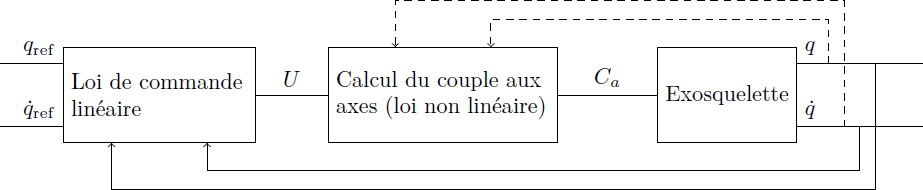
\includegraphics[width=\textwidth]{fig_06}
%Figure 6 
\caption{\label{fig:06}Schéma cinématique simplifié du mécanisme (représenté pour $\theta_{2}=\theta_{3}=0$ ) et figures de changement de base}
\end{figure}

\marginnote[1cm]{Toutes les liaisons sont supposées parfaites et les caractéristiques inertielles des solides sont les suivantes :
\begin{itemize}
\item étrier (2) : masse et inertie négligeables ;
\item toupie (3) : masse $m_{3}$, centre d'inertie $G_{3}$ tel que $\overrightarrow{O_{0} G_{3}}=L_{G_{3}} \vec{z}_{1}+H_{G_{3}} \vec{y}_{1}$. L'axe $\left(G_{3}, \vec{y}_{3}=\vec{y}_{2}\right)$ étant un axe de symétrie de révolution de la toupie (3), sa matrice d'inertie au point $G_{3}$ s'exprime dans la base $\mathcal{B}_{2}$ sous la forme $\mathcal{J}\left(G_{3}, 3\right)=\left[\begin{array}{ccc}A_{3} & 0 & 0 \\ 0 & B_{3} & 0 \\ 0 & 0 & A_{3}\end{array}\right]_{\mathcal{B}_{2}}$.
\end{itemize}}

Le système GyroLock, dont la modélisation est donnée figure \ref{fig:06}, est composé de trois solides :

\begin{itemize}
  \item le support, relié au stabilisateur (1) de repère associé $\mathcal{R}_{1}\left(O_{0}, \vec{x}_{1}, \vec{y}_{1}, \vec{z}_{1}\right)$, en liaison encastrement au point $O_{0}$ avec la table d'opération $(0)$;

  \item l'étrier (2) de repère associé $\mathcal{R}_{2}\left(A, \vec{x}_{2}, \vec{y}_{2}, \vec{z}_{1}=\vec{z}_{2}\right)$ tel que $\theta_{2}=\left(\vec{x}_{1}, \vec{x}_{2}\right)=\left(\vec{y}_{1}, \vec{y}_{2}\right)$;

  \item la toupie (3) de repère associé $\mathcal{R}_{3}\left(B, \vec{x}_{3}, \vec{y}_{2}=\vec{y}_{3}, \vec{z}_{3}\right)$ tel que $\theta_{3}=\left(\vec{x}_{2}, \vec{x}_{3}\right)=\left(\vec{z}_{2}, \vec{z}_{3}\right)$.

\end{itemize}

%Les figures de changement de base sont données figure \ref{fig:06}. 

Pour la modélisation des actions mécaniques extérieures, les hypothèses suivantes sont adoptées :

\begin{itemize}
  \item les actions mécaniques dues à la pesanteur sont négligées devant les effets dynamiques ;

  \item l'action mécanique transmise par la liaison encastrement entre les solides (0) et (1) est modélisée au point $G_{3} \operatorname{par}\left\{\mathcal{T}_{0 \rightarrow 1}\right\}=\left\{\begin{array}{c}X_{01} \vec{x}_{1}+Y_{01} \vec{y}_{1}+Z_{01} \vec{z}_{1} \\ L_{01} \vec{x}_{1}+M_{01} \vec{y}_{1}+N_{01} \vec{z}_{1}\end{array}\right\}_{G_{3}}$.

\end{itemize}

Le référentiel $\mathcal{R}_{0}\left(O_{0}, \vec{x}_{0}, \vec{y}_{0}, \vec{z}_{0}\right)$ lié à la table d'opération (0) est galiléen.
\fi

%Q 5.
\question{\label{q:05} Exprimer, dans la base $\mathcal{B}_{2}$, le moment cinétique au point $G_{3}$ du solide (3) en mouvement dans le référentiel $\mathcal{R}_{0}$, noté $\vec{\sigma}\left(G_{3}, 3 / 0\right)$.}
\ifprof
\begin{corrige}

\textbf{Au centre d'inertie} on a: $\overrightarrow{\sigma}(G_3,3/0) = \mathcal{I}(G_3,3)\overrightarrow{\Omega}(3/0)$ avec par \textbf{composition des vitesses} 

$\overrightarrow{\Omega}(3/0) = \underbrace{\overrightarrow{\Omega}(3/2)}_{\dot{\theta}_3 \overrightarrow{y}_2} + \underbrace{\overrightarrow{\Omega}(2/1)}_{\dot{\theta}_2\overrightarrow{z}_2} + \underbrace{\overrightarrow{\Omega}(1/0)}_{\overrightarrow{0}}$  la vitesse de rotation du solide (3) par rapport à (0) exprimée dans la base $\mathcal{B}_2$. Alors: $\boxed{\overrightarrow{\sigma}(G_3,3/0) = B_3\dot{\theta}_3\overrightarrow{y}_2 + A_3\dot{\theta}_2\overrightarrow{z}_2}$.
\end{corrige}
\else
\fi

%Q 6. 
\question{\label{q:06}En déduire, dans la base $\mathcal{B}_{2}$, le moment dynamique au point $G_{3}$ du solide (3) en mouvement dans le référentiel $\mathcal{R}_{0}$, noté $\vec{\delta}\left(G_{3}, 3 / 0\right)$.}
\ifprof
\begin{corrige}
Toujours \textbf{au centre d'inertie} on a 

$\boxed{\overrightarrow{\delta}(G_3,3/0) = \left. \dfrac{\mathrm{d}\overrightarrow{\sigma}(G_3,3/0)}{\mathrm{d}t} \right|_{0} = -B_3\dot{\theta}_2\dot{\theta}_3\overrightarrow{x}_2 + B_3 \ddot{\theta}_3\overrightarrow{y}_2 + A_3\ddot{\theta}_{2}\overrightarrow{z}_2}$. 
\end{corrige}
\else
\fi

%Q 7. 
\question{\label{q:07}Après avoir clairement précisé le système isolé et le théorème utilisé, exprimer $L_{01}, M_{01}$ et $N_{01}$ en fonction de $\theta_{2}, \theta_{3}$ (et leurs dérivées temporelles), $A_{3}$ et $B_{3}$.}
\ifprof

\begin{figure}[!h]
\centering
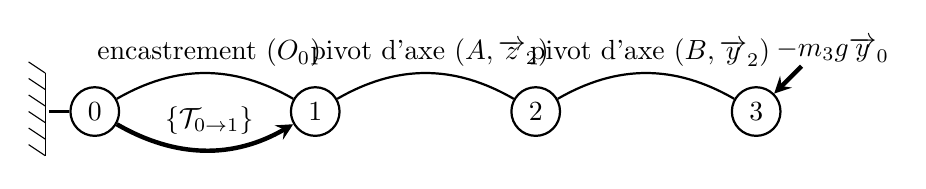
\begin{tikzpicture}[scale=.7]

% définition des styles
\tikzstyle{arc}=[-,thick]
\tikzstyle{pointille}=[dashed,thick]
\tikzstyle{cercle}=[circle,text centered,draw,thick]
\tikzstyle{fleche}=[->,ultra thick,>=stealth]

% les ellipses
\node [cercle] (0) at (0,0) {0};
\node [cercle] (1) at (4cm,0cm){1};
\node [cercle] (2) at (8cm,0cm){2};
\node [cercle] (3) at (12cm,0cm){3};
\node (0a) at (-1cm,0cm){} ;
\node (3a) at (13cm,1cm){} ;

% les arcs
\draw[arc] (0) to[bend left] node[pos=0.3,above,yshift=0mm,xshift=5mm]{encastrement $(O_0)$} (1);
\draw[arc] (1) to[bend left] node[pos=0.3,above,yshift=0mm,xshift=5mm]{pivot d'axe $(A,\overrightarrow{z}_2)$} (2);
\draw[arc] (2) to[bend left] node[pos=0.3,above,yshift=0mm,xshift=5mm]{pivot d'axe $(B,\overrightarrow{y}_2)$} (3);


\draw[fleche] (0) to[bend right] node[pos=0.3,above,yshift=0mm,xshift=5mm]{$\{\mathcal{T}_{0 \to 1}\}$} (1);
\draw[fleche] (3a) to node[pos=0.3,above,yshift=0mm,xshift=5mm]{$-m_3 g \overrightarrow{y}_0$} (3);


% Bâti
\draw[] (-0.9cm,0.7cm) to node[]{} (-0.9cm,-0.8cm) ;
%%%\draw[] (-1.2cm,1.2cm) to node[]{} (-0.9cm,1cm) ;
\draw[] (-1.2cm,0.9cm) to node[]{} (-0.9cm,0.7cm) ;
\draw[] (-1.2cm,0.6cm) to node[]{} (-0.9cm,0.4cm) ;
\draw[] (-1.2cm,0.3cm) to node[]{} (-0.9cm,0.1cm) ;
\draw[] (-1.2cm,0.0cm) to node[]{} (-0.9cm,-0.2cm) ;
\draw[] (-1.2cm,-0.3cm) to node[]{} (-0.9cm,-0.5cm) ;
\draw[] (-1.2cm,-0.6cm) to node[]{} (-0.9cm,-0.8cm) ;
\draw[arc] (0a) to node[]{} (0) ;

\end{tikzpicture}
\end{figure}
\begin{corrige}
Pour la clarté on propose le graphe des liaisons ci-desus avec les différentes actions mécaniques qui s'exercent sur le système.


On isole le système $\Sigma = \{ 1+2+3 \}$ soumis à:
\begin{itemize}
\item[•] l'action de (0) sur (1) en $G_3$: $\{\mathcal{T}_{0 \to 1}\}$;
\item[•] l'action du poids en $G_3$: $-m_3 g \overrightarrow{y}_0$.
\end{itemize}

On applique le \textbf{théorème du moment dynamique au système $\Sigma$ au point $G_3$}:

$$ \boxed{\overrightarrow{\delta}(G_3,\Sigma/0) = L_{01}\overrightarrow{x}_1 + M_{01}\overrightarrow{y}_1 + N_{01}\overrightarrow{z}_1} $$

Or $\overrightarrow{\delta}(G_3,\Sigma/0) = \overrightarrow{\delta}(G_3,3/0)$ car \textbf{on néglige les effets dynamiques de (1) et (2)}. Par conséquent:
$ -B_3\dot{\theta}_2\dot{\theta}_3\overrightarrow{x}_2 + B_3 \ddot{\theta}_3\overrightarrow{y}_2 + A_3\ddot{\theta}_{2}\overrightarrow{z}_2 = L_{01}\overrightarrow{x}_1 + M_{01}\overrightarrow{y}_1 + N_{01}\overrightarrow{z}_1$.

Dans la base $\mathcal{B}_1$ on obtient le système d'équations:

$$
\left\{
\begin{array}{ll}
L_{01}(t) = - B_3 \dot{\theta}_3\dot{\theta}_2 \cos(\theta_2(t)) - B_3 \ddot{\theta}_3 \sin(\theta_2)  \\
M_{01}(t) = - B_3 \dot{\theta}_3\dot{\theta}_2 \sin(\theta_2(t)) + B_3 \ddot{\theta}_3 \cos(\theta_2) \\
N_{01}(t) = A_3 \ddot{\theta}_2(t)
\end{array}
\right.
$$
 
\end{corrige}
\else
\fi

\ifprof
\else
Lorsque la toupie (3) tourne avec une vitesse constante $\omega_{3}$ par rapport à l'étrier (2), l'expression des moments $L_{01}, M_{01}$ et $N_{01}$ est la suivante :
$
\left\{\begin{array}{l}
L_{01}(t)=-c_{x}(t) \cos \theta_{2}(t) \\
M_{01}(t)=-c_{x}(t) \sin \theta_{2}(t) \\
N_{01}(t)=A_{3} \ddot{\theta}_{2}(t)
\end{array}\right.
$.

où $c_{x}(t)=B_{3} \omega_{3} \dot{\theta}_{2}(t)=K_{3} \dot{\theta}_{2}(t)$ correspond à l'effet gyroscopique.

L'action du cœur sur le stabilisateur est modélisée par un glisseur de résultante $\vec{R}_{c \rightarrow 1}=f_{c} \vec{y}_{1}$ au point $P$ tel que $\overrightarrow{O_{0} P}=L \vec{z}_{1}$.

Les moments $L_{01}, M_{01}$ et $N_{01}$ doivent rester faibles afin de limiter les déformations de l'attache reconfigurable liant le stabilisateur (1) à la table d'opération (0). 
\fi

%Q 8. 
\question{\label{q:08}En supposant que la toupie (3) tourne à vitesse constante par rapport à l'étrier (2), exprimer $\dot{\theta}_{2}$ en fonction de $K_{3}, \theta_{2}, f_{c}$ et $L-L_{G_{3}}$ permettant de garantir $L_{01}=0$ et de compenser l'effet de l'effort cardiaque $f_{c}$.}
\ifprof

\begin{figure}[!h]
\centering
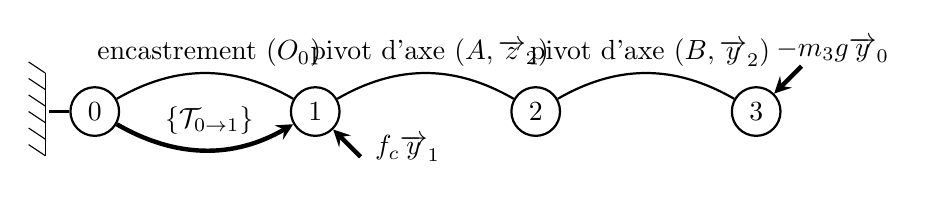
\begin{tikzpicture}[scale=.7]

% définition des styles
\tikzstyle{arc}=[-,thick]
\tikzstyle{pointille}=[dashed,thick]
\tikzstyle{cercle}=[circle,text centered,draw,thick]
\tikzstyle{fleche}=[->,ultra thick,>=stealth]

% les ellipses
\node [cercle] (0) at (0,0) {0};
\node [cercle] (1) at (4cm,0cm){1};
\node [cercle] (2) at (8cm,0cm){2};
\node [cercle] (3) at (12cm,0cm){3};
\node (0a) at (-1cm,0cm){} ;
\node (3a) at (13cm,1cm){} ;
\node (1a) at (5cm,-1cm){} ;

% les arcs
\draw[arc] (0) to[bend left] node[pos=0.3,above,yshift=0mm,xshift=5mm]{encastrement $(O_0)$} (1);
\draw[arc] (1) to[bend left] node[pos=0.3,above,yshift=0mm,xshift=5mm]{pivot d'axe $(A,\overrightarrow{z}_2)$} (2);
\draw[arc] (2) to[bend left] node[pos=0.3,above,yshift=0mm,xshift=5mm]{pivot d'axe $(B,\overrightarrow{y}_2)$} (3);


\draw[fleche] (0) to[bend right] node[pos=0.3,above,yshift=0mm,xshift=5mm]{$\{\mathcal{T}_{0 \to 1}\}$} (1);
\draw[fleche] (3a) to node[pos=0.3,above,yshift=0mm,xshift=5mm]{$-m_3 g \overrightarrow{y}_0$} (3);
\draw[fleche] (1a) to node[pos=0.3,yshift=0mm,xshift=7mm]{$f_c \overrightarrow{y}_1$} (1);


% Bâti
\draw[] (-0.9cm,0.7cm) to node[]{} (-0.9cm,-0.8cm) ;
%%%\draw[] (-1.2cm,1.2cm) to node[]{} (-0.9cm,1cm) ;
\draw[] (-1.2cm,0.9cm) to node[]{} (-0.9cm,0.7cm) ;
\draw[] (-1.2cm,0.6cm) to node[]{} (-0.9cm,0.4cm) ;
\draw[] (-1.2cm,0.3cm) to node[]{} (-0.9cm,0.1cm) ;
\draw[] (-1.2cm,0.0cm) to node[]{} (-0.9cm,-0.2cm) ;
\draw[] (-1.2cm,-0.3cm) to node[]{} (-0.9cm,-0.5cm) ;
\draw[] (-1.2cm,-0.6cm) to node[]{} (-0.9cm,-0.8cm) ;
\draw[arc] (0a) to node[]{} (0) ;

\end{tikzpicture}
\end{figure}

\begin{corrige}
Le nouveau graphe de liaison est donné ci-dessus.

On reprend la stratégie précédente mais on ajoute le moment en $G_3$ provoqué par la résultante $\overrightarrow{R}_{c \to 1}$ en $P$: $\overrightarrow{M}\left(G_3,\overrightarrow{R}_{c \to 1}\right) = \overrightarrow{G_3 P} \wedge f_c\overrightarrow{y}_1 = (L - L_{G_3})f_c \overrightarrow{x}_1$. L'équation du mouvement précédente écrite dans la base $\mathcal{B}_1$ donne alors le système d'équations:

$$
\left\{
\begin{array}{ll}
L_{01}(t) + (L - L_{G_3})f_c = - K_3\dot{\theta}_2 \cos(\theta_2(t)) \\
M_{01}(t) = - K_3\dot{\theta}_2 \sin(\theta_2(t)) \\
N_{01}(t) = A_3 \ddot{\theta}_2(t)
\end{array}
\right.
$$

En particulier si on veut $L_{01} = 0$ alors $\boxed{\dot{\theta}_2 = - \dfrac{(L - L_{G_3})f_c}{K_3\cos(\theta_2(t))}}$ en faisant attention à avoir $|\theta_2| < \dfrac{\pi}{2}$.
 

\end{corrige}
\else
\fi

%Q 9. 
\question{\label{q:09}Donner une condition sur l'angle $\theta_{2}$ et sur l'accélération angulaire $\ddot{\theta}_{2}$ afin que les moments $M_{01}$ et $N_{01}$ soient faibles.}
\ifprof
\begin{corrige}
D'après le système d'équations de la question précédente:
\begin{itemize}
\item si on veut $N_{01} \to 0$ alors il faut $\ddot{\theta}_2 \to 0$ (accélération angulaire très faible);
\item si on veut $M_{01} \to 0$ alors en prenant $\theta_2 \ll 1$rad on a une chance d'y arriver.
\end{itemize} 

\textbf{Remarque:} d'après la question 8, si on prend $\omega_3$ très grand alors $\dot{\theta}_2$ est potentiellement très petit ce qui aide à \og écraser \fg{} $M_{01}$.
\end{corrige}
\else
\fi

\ifprof
\else
L'étrier (2) doit être piloté en vitesse de rotation pour que l'effet gyroscopique $c_{x}(t)=K_{3} \dot{\theta}_{2}(t)$ compense l'effet de l'effort cardiaque. La campagne expérimentale présentée en partie I a permis de déterminer que la fréquence fondamentale de l'effort cardiaque $f_{c}(t)$ est de $1,5 \mathrm{~Hz}$.

La réponse de l'étrier (2) sera considérée comme suffisamment réactive si le temps de réponse à $5 \%$ de la vitesse $\dot{\theta}_{2}(t)=\omega_{2}(t)$ pour une consigne $\dot{\theta}_{c 2}(t)=\omega_{c 2}(t)$ en échelon est d'un ordre inférieur à la demi-période du signal perturbateur $f_{c}(t)$.

La réponse expérimentale à un échelon de vitesse $\omega_{c 2}(t)$ d'amplitude $2000 \mathrm{deg} \cdot \mathrm{s}^{-1}$ est représentée figure \ref{fig:07}.

\begin{figure}[!h]
\centering
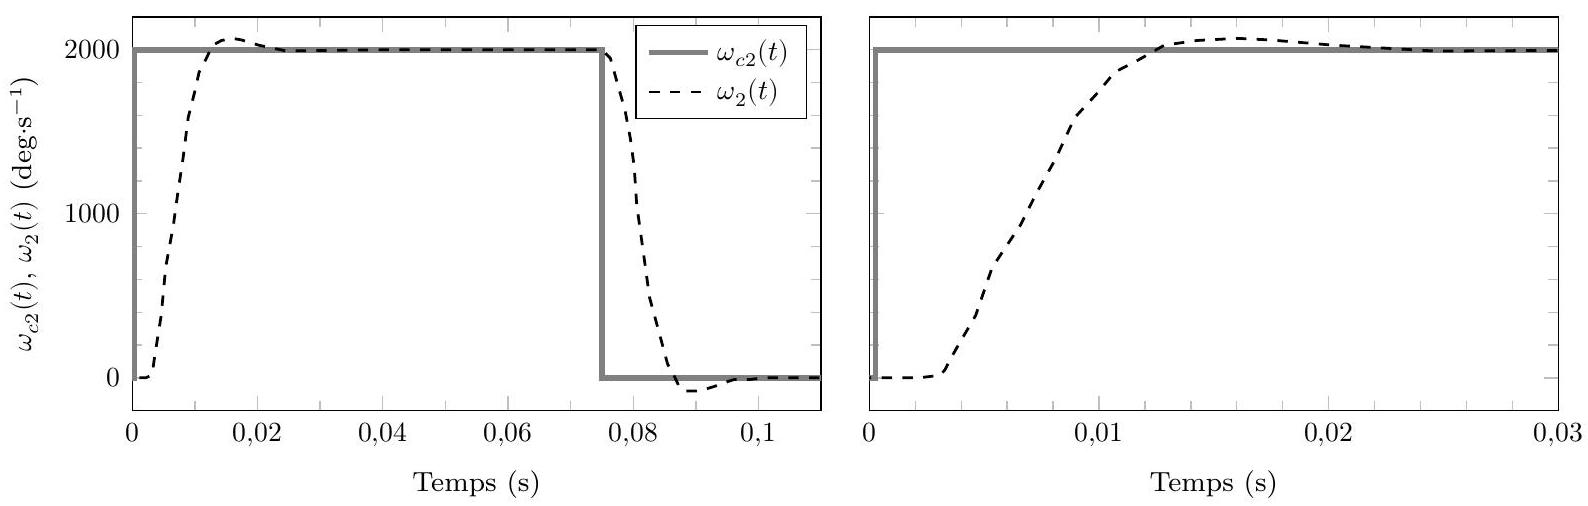
\includegraphics[width=\textwidth]{fig_07}
%Figure 7 
\caption{\label{fig:07}Réponse expérimentale de l'étrier et consigne associée (à droite, zoom sur le régime transitoire)}
\end{figure}

Les transformées de Laplace de $\omega_{2}(t), \omega_{c 2}(t), \theta_{2}(t)$ et $c_{x}(t)$ sont notées $\Omega_{2}(p), \Omega_{c 2}(p), \theta_{2}(p)$ et $C_{x}(p)$.
\fi

%Q 10. 
\question{\label{q:10}Vérifier que la condition de réactivité énoncée ci-dessus est respectée. Justifier que la fonction de transfert de l'étrier (2) $H_{2}(p)=\frac{\Omega_{2}(p)}{\Omega_{c 2}(p)}$ peut alors être approchée par un gain statique $K_{2}$ de valeur à préciser. Il faut s'assurer que la position $\theta_{2}$ de l'étrier (2) ne s'éloigne pas trop de sa position de référence $\theta_{2}^{*}=0$. Le non-respect de cette condition, appelé dérive de l'étrier, génère un moment parasite $M_{01}$ responsable d'un déplacement du point $P$ selon $\vec{x}_{1}$.}
\ifprof
\begin{corrige}
La période du signal perturbateur est $T_c = \dfrac{1}{f_c}$, donc la demi période est $\dfrac{T_c}{2} = \dfrac{1}{2f_c} = 0,33$s.\\

Si on veut respecter la condition de réactivité il faut donc que le temps de réponse à 5\% soit inférieur à $0,033$s.\\

On lit sur le graphe de droite en figure 7 que la valeur finale est atteinte avant 0,03s donc le temps de réponse à 5\% est d'autant plus petit et \textbf{la condition de réactivité est respectée}.\\

Si on considère le système très réactif, comme celui-ci est précis on peut supposer que $\boxed{H_2(p) = \dfrac{\Omega_2(p)}{\Omega_{c2}(p)} = K_2 = 1}$.
\end{corrige}
\else
\fi



